\documentclass{article}


\usepackage[final, nonatbib]{neurips_2023}

\usepackage[utf8]{inputenc} % allow utf-8 input
\usepackage[T1]{fontenc}    % use 8-bit T1 fonts
\usepackage{hyperref}       % hyperlinks
\usepackage{url}            % simple URL typesetting
\usepackage{booktabs}       % professional-quality tables
\usepackage{amsfonts}       % blackboard math symbols
\usepackage{nicefrac}       % compact symbols for 1/2, etc.
\usepackage{microtype}      % microtypography

\usepackage{graphicx}
\usepackage{caption}
\usepackage{subcaption}
\graphicspath{{images/}}
\usepackage{multirow}
\usepackage[table,xcdraw]{xcolor}
\usepackage{subfiles} % Best loaded last in the preamble


\title{Feature Manipulation for DDPM based Change Detection}


\author{%
  Daehyeon Choi\\
  20210716\\
  \And
  Jeongho Son\\
  20210979\\
  \And
  Seunghun Oh\\
  20190439\\
}


\begin{document}


\maketitle

\begin{abstract}
  Change Detection is a classic task of computer vision that receives a bi-temporal image pair as an input and separates the semantically changed and unchanged regions of it. Diffusion Model is not only used in Image Synthesis, but also used as a feature extractor and has been applied to various downstream tasks. Using this, a feature map is extracted from the pre-trained diffusion model from the large-scale data set and changes are detected through the additional network in previous. 
  On the one hand, the current Diffusion-based Change Detection approach focuses only on how to extract a good feature map with the Diffusion Model, and obtains and uses difference without further adjustment to the created feature map. Our method focuses on manipulating the feature map extracted from the Diffusion Model to be more semantically useful, and for this, we propose two methods: Feature Attention and FDAF. Our model with Feature Attention achieved state-of-the-art F1 score (91.52) and IoU (84.36) on LEVIR-CD dataset. All our codes are available at \href{https://github.com/choidaedae/POSTECH-CSED538/}{https://github.com/choidaedae/POSTECH-CSED538/}.
\end{abstract}


\section{Introduction}

\subfile{subfiles/introduction.tex}


\section{Method}

\begin{figure}[h]
  \centering
  \begin{subfigure}[b]{0.4\linewidth}
      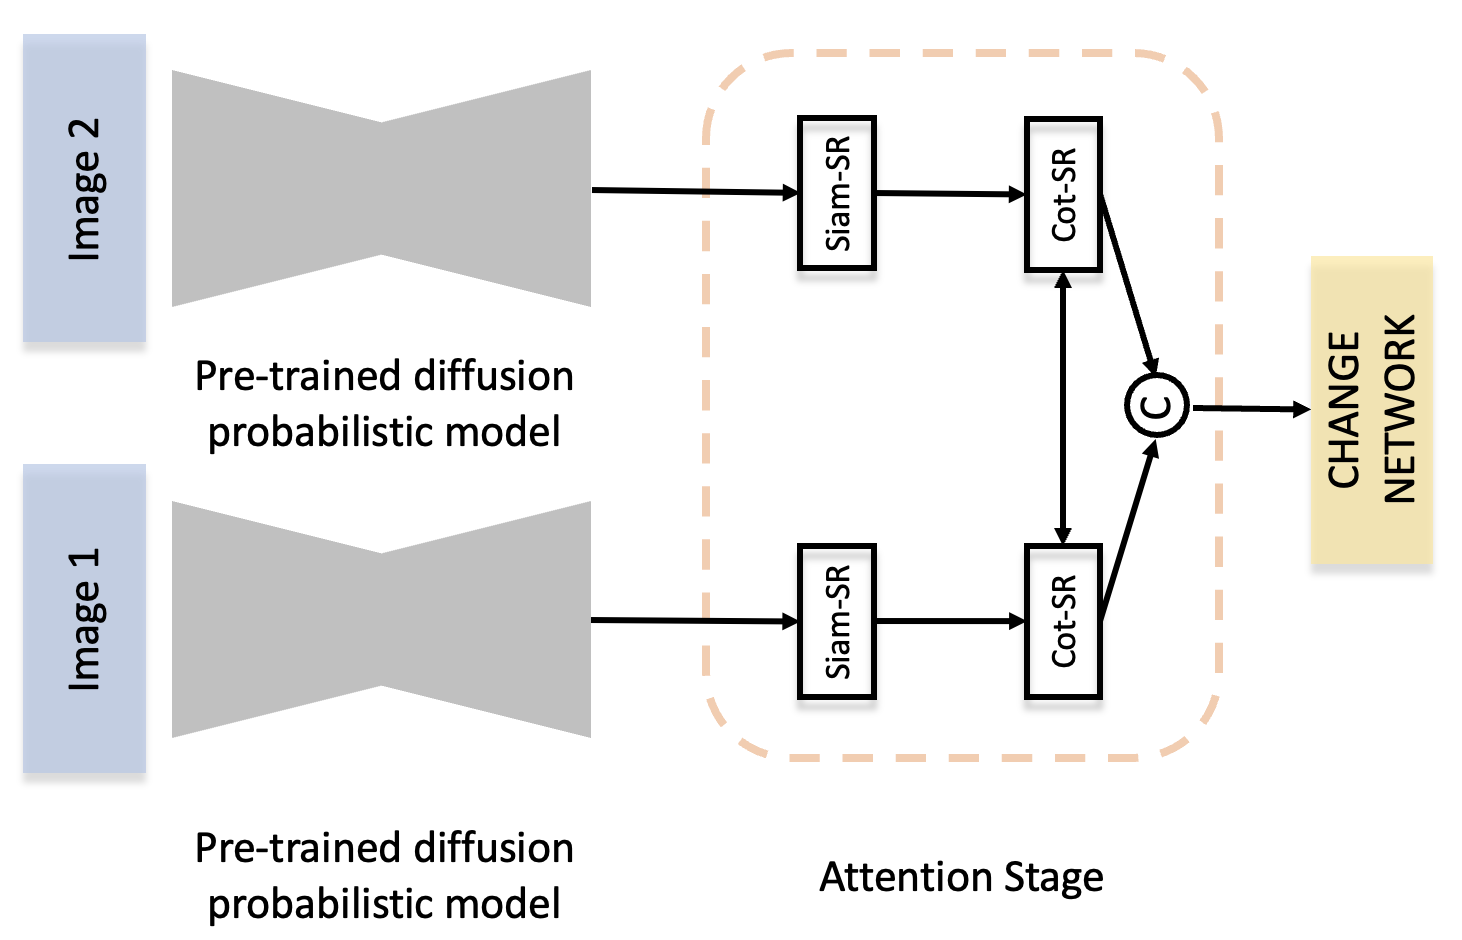
\includegraphics[width=\linewidth]{baseline_with_attention.png}
      \caption{Attention based model}
      \label{fig:baseline_with_attention}
  \end{subfigure}
  \hspace{0.1\textwidth}
  \begin{subfigure}[b]{0.4\linewidth}
      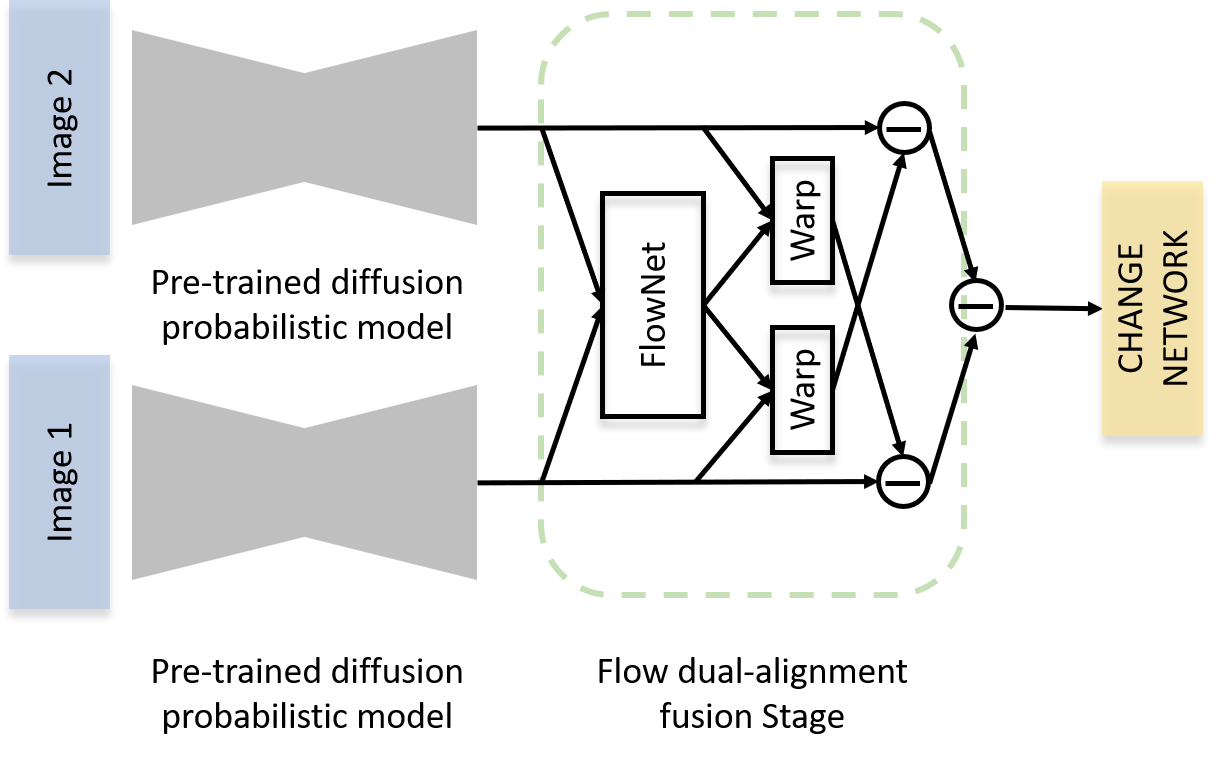
\includegraphics[width=\linewidth]{baseline_with_fdaf.png}
      \caption{FDAF based model}
      \label{fig:baseline_with_fdaf}
  \end{subfigure}
  \caption{Structure of the baseline model with attention and FDAF}
  \label{fig:baseline_with_attention_and_fdaf}
\end{figure}

\subsection{Feature Attention}

\subfile{subfiles/method_attention.tex}

\subsection{FDAF}

\subfile{subfiles/method_fdaf.tex}


\section{Experiment}

\subfile{subfiles/experiment.tex}


\section{Conclusion}

\subfile{subfiles/conclusion.tex}

\newpage


\bibliographystyle{splncs04}
\bibliography{reference}

\end{document}